
	\begin{figure}
		\centering
		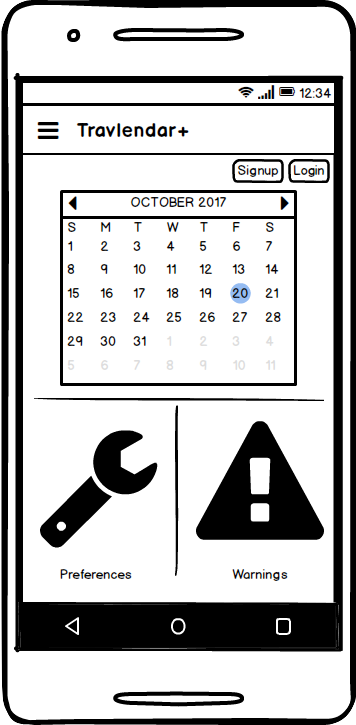
\includegraphics[width=0.6\linewidth]{mockups/Homepage}
		\caption{Travlendar+ homepage.  
		}
	\label{fig:homepage}
	\begin{center}
		To pursue our aim of realizing a user-friendly and light app, we decided to provide the main functions directly in the homepage. Indeed, from this page, a guest can reach the sign up form, a user can log himself in,can insert a meeting by tapping onto a day in the calendar,can manage his preferences and even access the warnings. \\ 
	\end{center}
	\end{figure}


				
				
	\begin{figure}
	\centering
	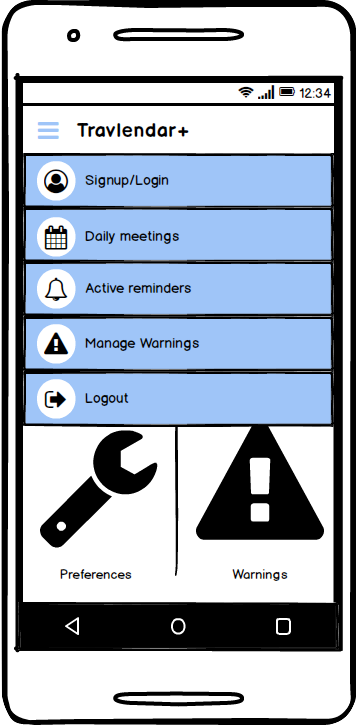
\includegraphics[width=0.6\linewidth]{mockups/QuickMenu}
	\caption{Quick access menu.}
	\label{fig:quickmenu}
	\begin{center}
		We thought about a quick menu to collect some secondary functions, to make them easily reachable. By tapping on the left high corner of the app. people has the opportunity to either register or log in themselves, to view only the meetings of the current day, to access the reminders they setted up, to manage the warnings and to logout themselves if they are already logged in.
	\end{center}
	\end{figure}

	\begin{figure}
		\centering
		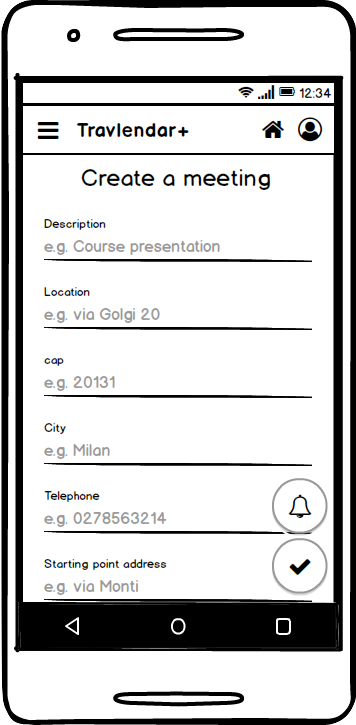
\includegraphics[width=0.6\linewidth]{mockups/CreateMeeting}
		\caption{Meeting creation page.}
		\label{fig:createmeeting}
		\begin{center}
			This page is a very simple form, which allows the user to finalize the creation of a meeting by filling it in all its fields. 
			The house-logo in the  right corner,on the top band and near the application name, represent the return-to-homepage icon. 
		\end{center}
	\end{figure}

	\begin{figure}
	\centering
	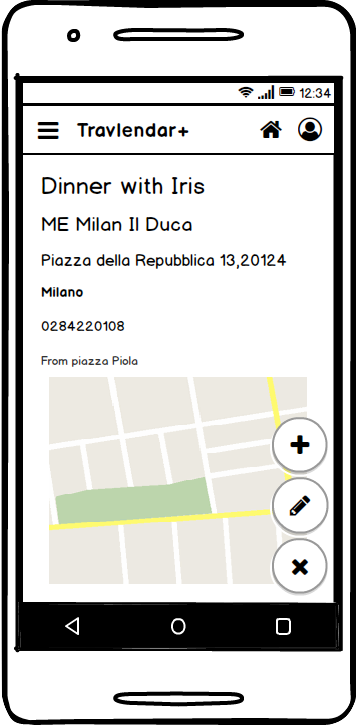
\includegraphics[width=0.6\linewidth]{mockups/MeetingView}
	\caption{Meeting view page. }
	\label{fig:meeting-view}
	\begin{center}
		This screen wants to provide all the useful information related to a meeting already registered in the system. First details provided, in the highest portion of the page, regard the meeting location and the route to reach the appointment, further information are located below. In addition, on the right part of the screen, there are quick access buttons: the "plus" icon allows the user to add a reminder for the event, the "pencil" icon is to change meeting details and the "x" button provides deletion function. 
	\end{center}
	\end{figure}

	\begin{figure}
		\centering
		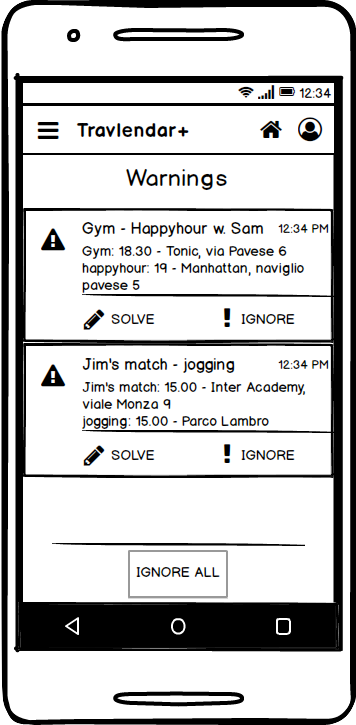
\includegraphics[width=0.6\linewidth]{mockups/Warnings}
		\caption{Warnings page}
		\label{fig:warnings}
		\begin{center}
			The warnings page has the role to summarize and notify all the conflict among meetings which involv the user's appointments. Every warning is represent by a dialog which points out the meetings that generate the conflict and which has two buttons, one to ignore the warning and other one to solve it by modifying the conflictual meetings. 
			To prevent too much user's clicks, is provided an "ignore all" button, which is equivalent to tap "ignore" for each warning in the list. 
		\end{center}
	\end{figure}

	\begin{figure}
		\centering
		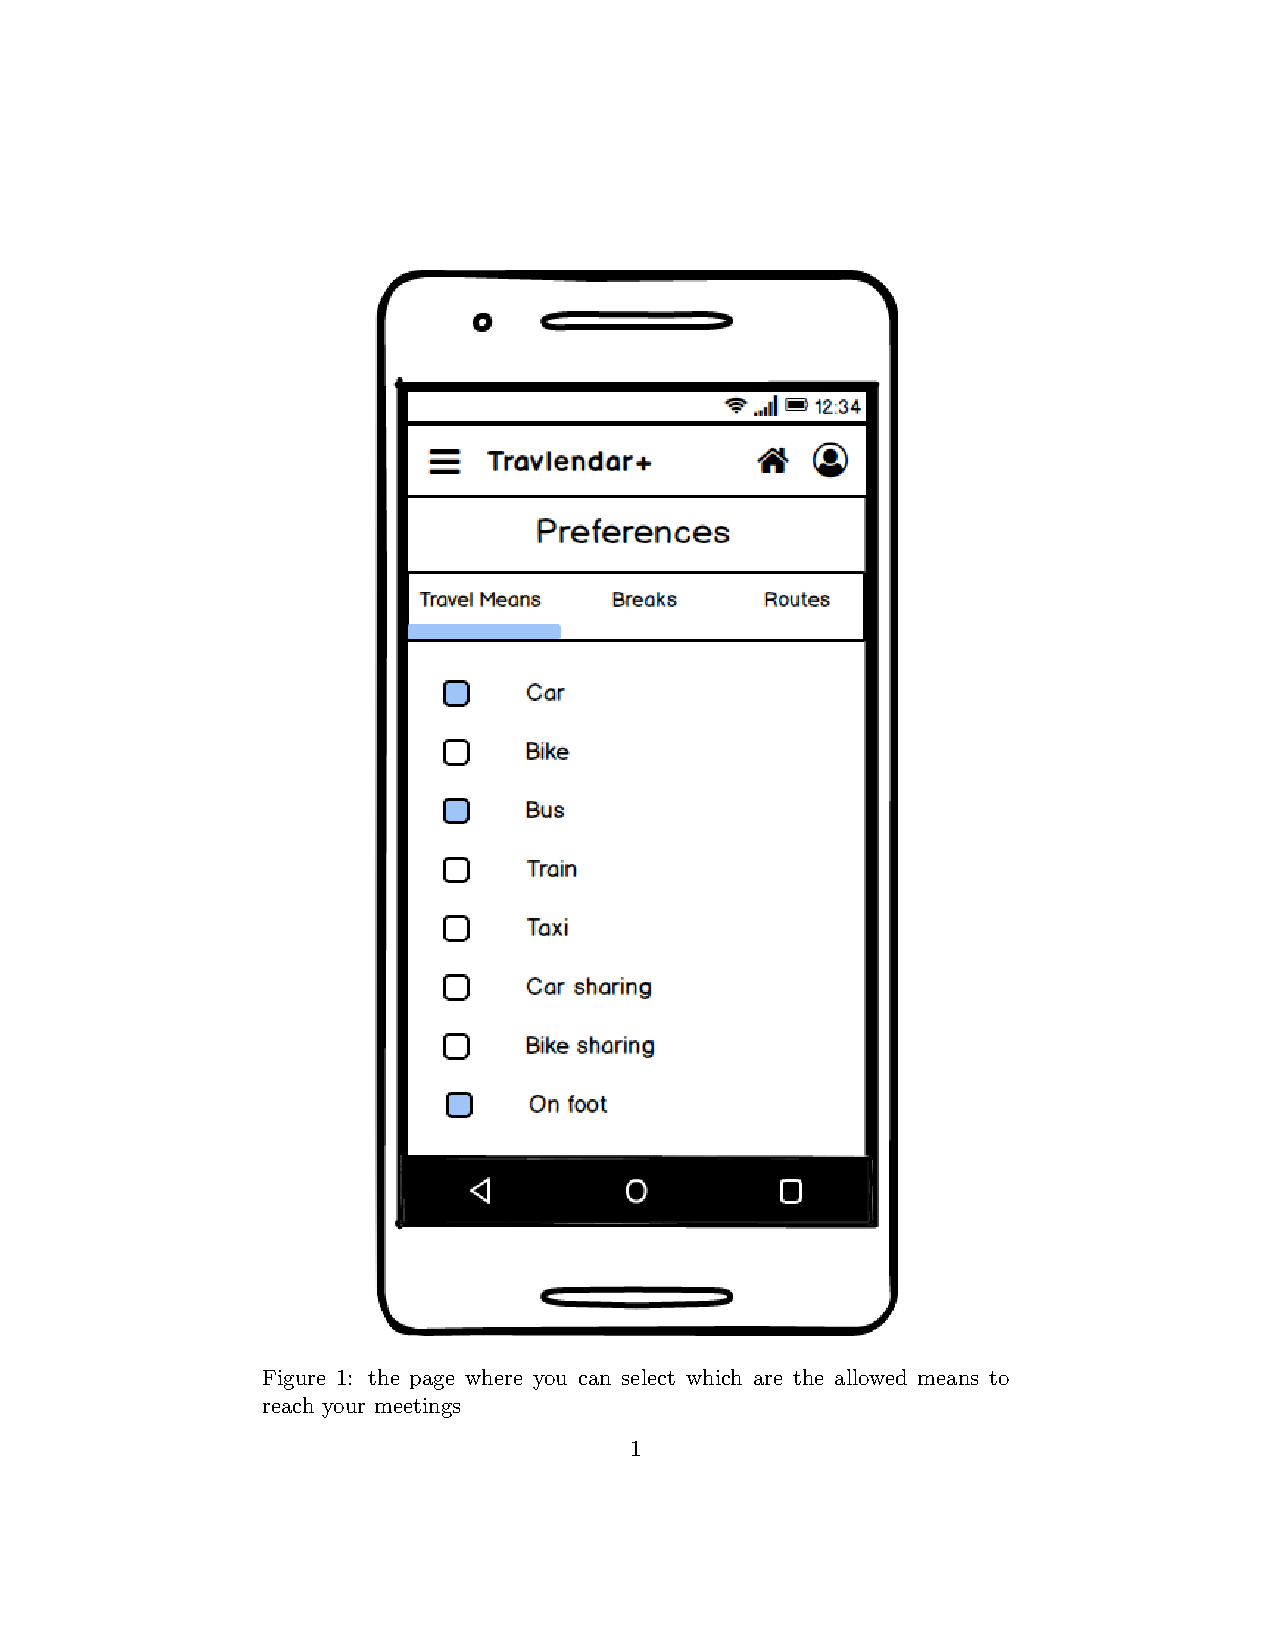
\includegraphics[width=0.6\linewidth]{mockups/PreferencesTravelMeans}
		\caption{Travel mean preferences page.}
		\label{fig:preferencestravelmeans}
			\begin{center}
			This is a very simple page with a minimalistic design, not to uselessly load the application. However this basical view provides all the function which the user needs to select his preferences on the transports for his travels. 
			Please note that the preference section can be switched by tapping on an specific topic just below the "Preferences" band.
			\end{center}
	\end{figure}

		\begin{figure}
		\centering
		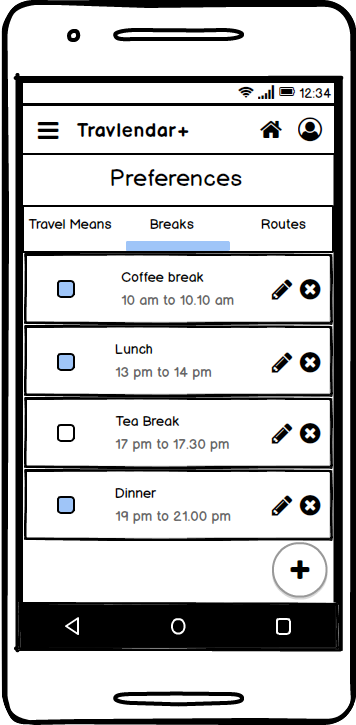
\includegraphics[width=0.6\linewidth]{mockups/PreferencesBreaks}
		\caption{Break preferences page.}
		\label{fig:preferencesbreaks}
		\begin{center}
			The breaks page consists in a list of events, that represents pauses, organized in order of generation and labeled by the type of the break. For every break are provided both the starting and the ending time, a "pencil" button to allow modifications and a "x" button to remove it. In addition, thanks to the fact that we decided to make the breaks general, that means not related to a specific day, the user has the faculty to either pick or unpick them to activate or deactivate them. 
		\end{center}
		\begin{center}
			
		\end{center}
	\end{figure}
	
		\begin{figure}
		\centering
		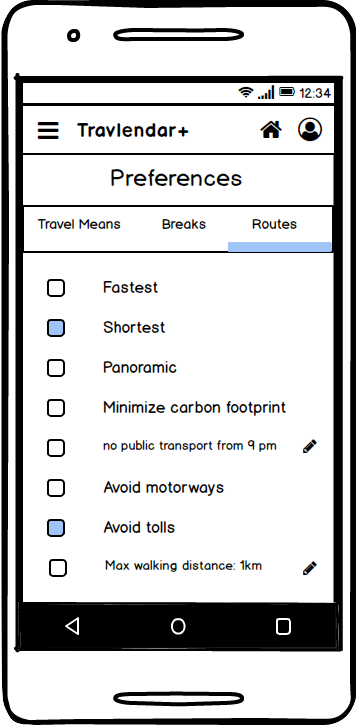
\includegraphics[width=0.6\linewidth]{mockups/PreferencesRoutes}
		\caption{Route preferences page}
		\label{fig:preferencesroutes}
		\begin{center}
			The route preferences page is very similar to the Travel mean preferences page. The style is the same and the opportunity to pick or unpick elements too, however there are differences. Some of the preferences in this section are mutal exclusive, so the user is prevented to select more than one of them (for instance a user can select either the shortest route or the fastest). Moreover, some selection element has customizable details, they are represented with a pencil logo on the right, and can be managed by the user to best fit his preferences ( for example the user can select after which hour he do not want to use public transports).
		\end{center}
	\end{figure}
	